\section{Theorie}
\label{sec:Theorie}


Ein Geiger-Müller-Zählrohr ist eine Apparatur, mit der die Intensität ionisierter Strahlung gemessen werden kann.
Im folgenden werden Aufbau, Charakteristik und Totzeit erklärt.
\subsection{Aufbau und Funktionsweise}
Ein schematischer Aufbau ist in \hyperref[fig:Aufbau1]{Abbildung \ref{fig:Aufbau1}} dargestellt.
\begin{figure} [H]
    \center
    \caption{Schematischer Aufbau eines Zählrohres}\label{fig:Aufbau1}
    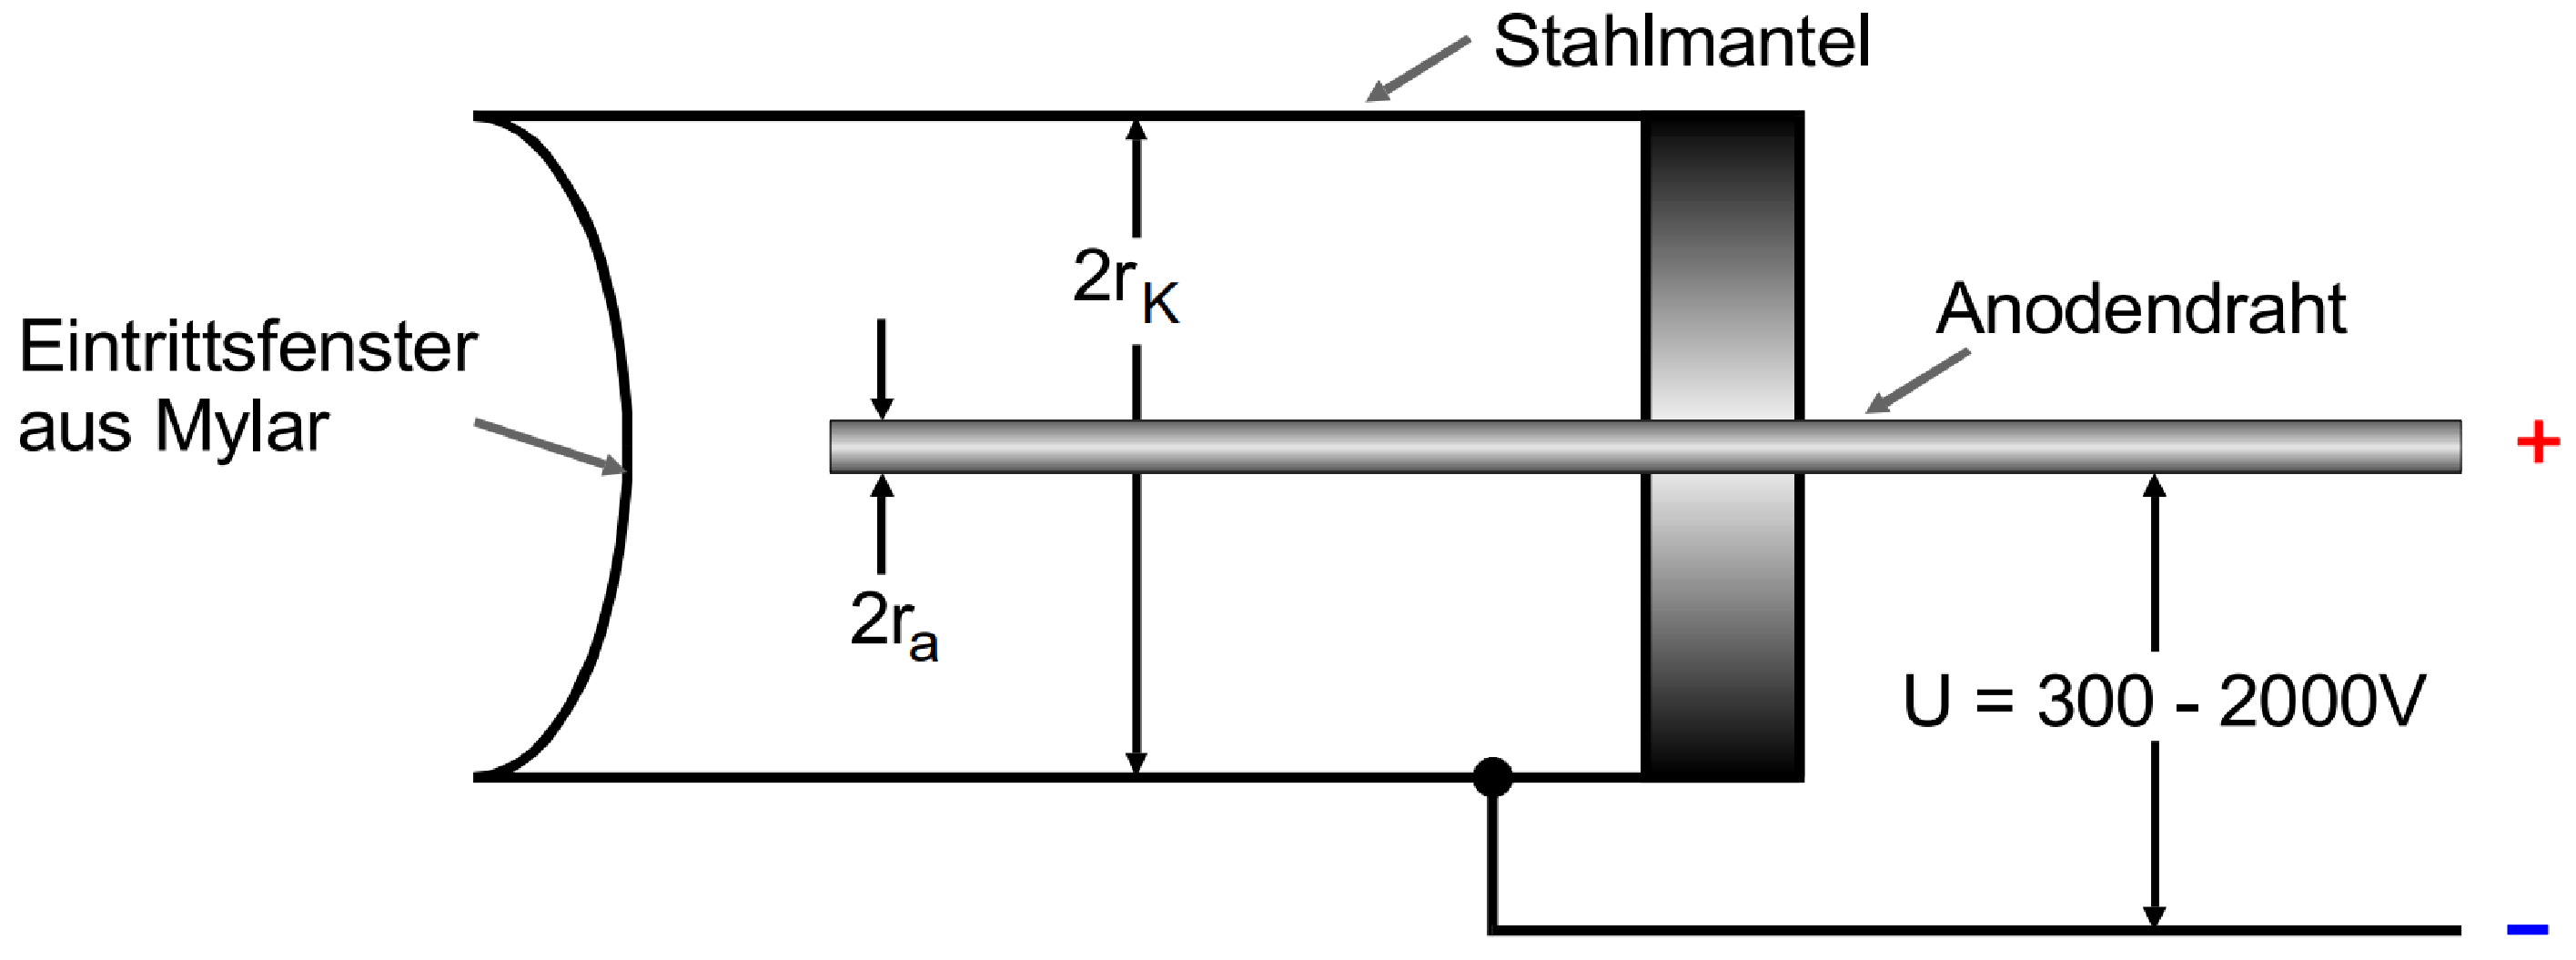
\includegraphics[width=0.7\linewidth]{pictures/Aufbau1.pdf}
\end{figure}
Im Wesentlichen besteht das Zählrohr aus einem Kathodenzylinder und einem Anodendraht im Inneren.
Dabei ist der Zylinder mit einem Gasgemisch befüllt.
Wird eine äußere Spannung angelegt, bildet sich ein radialsymmetrisches Feld zwischen Kathode und Anode.
Das Feld hat den Wert
\begin{equation}
    E(r)=\frac{U}{r \ln \left(r_{k} / r_{a}\right)}.
\end{equation}
Um nun ionisierte Strahlung messen zu können, müssen also diese Teilchen in das Zählrohr eintreten.
Dabei wird sich das Teilchen durch Ionisationsakte so lange durch die Röhre bewegen, bis die Energie aufgebraucht ist.
Dadurch werden im Inneren Elektronen und Ionen frei. Beim Auftreffen auf der Anode werden dann elektrische Impulse erzeugt.
Diese lassen sich messen und somit Rückschlüsse auf die Strahlung geben.
Jedoch sind die Vorgänge innerhalb des Zählrohres stark abhängig von der angelegten Spannung.
\begin{figure}
    \center
    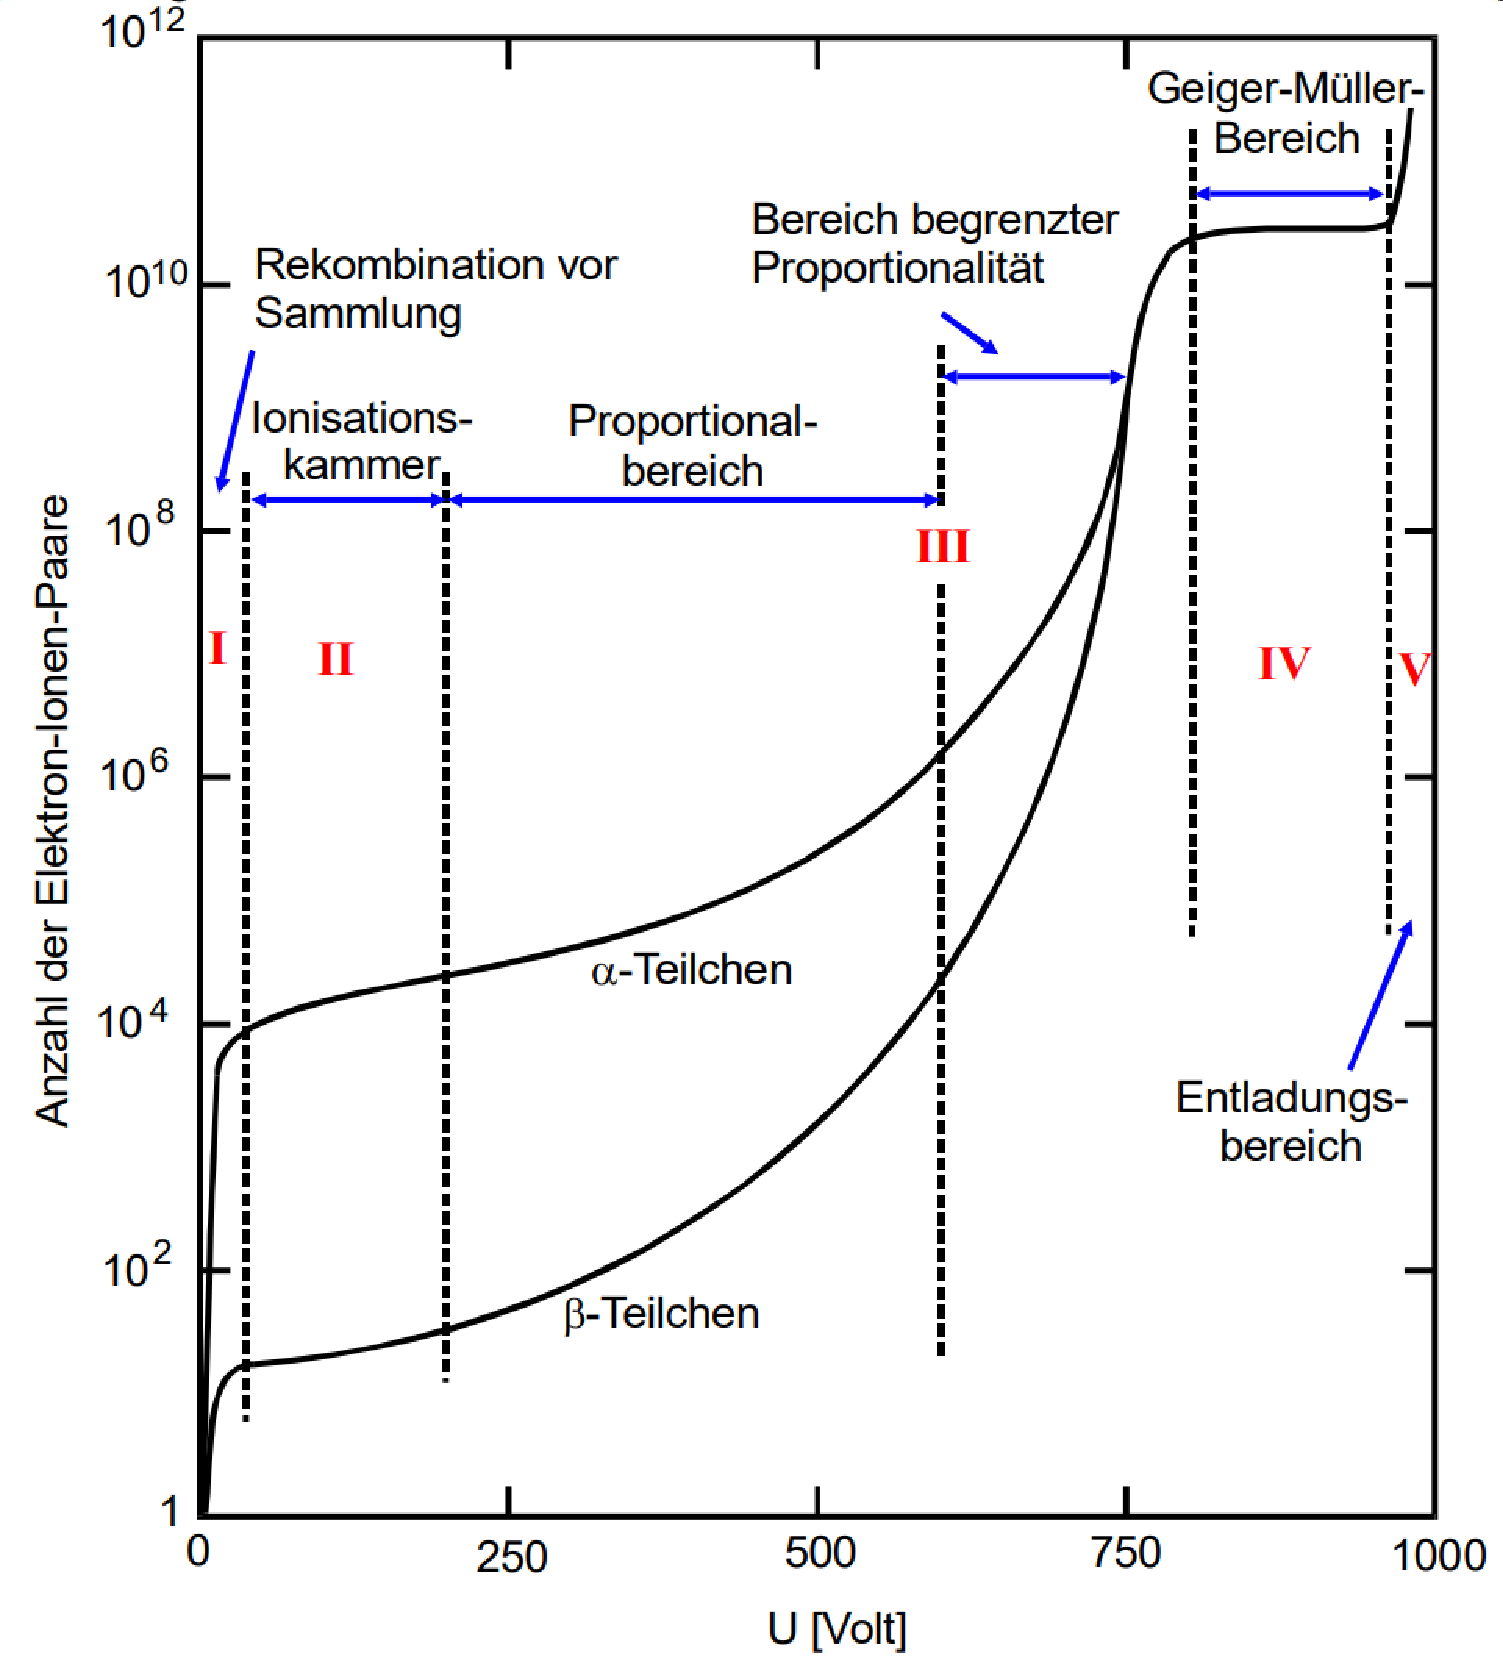
\includegraphics[width=0.5\linewidth]{pictures/Diagramm1.pdf}
    \caption{Anzahl der erzeugten Elektron-Ionenpaare als Funktion der Spannung U bei einem Proportionalzählrohr.}\label{fig:Diagramm1}
\end{figure}
Dieses ist in \hyperref[fig:Diagramm1]{Abbildung \ref{fig:Diagramm1}} schematisch dargestellt.
Ist die Spannung gering, geht bereits vor dem Erreichen der Elektronen ein Großteil durch Rekombination verloren.
Wird die Spannung erhöht, sind die Wahrscheinlichkeit für Rekombination drastisch ab (Bereich 1).
Bereich 2 kann also bereits verwendet werden um hohe Strahlungsintensitäten zu messen.
So eine Apparatur wird üblicherweise \textit{Ionisationskammer} genannt.
In Bereich 3 sind die freigesetzten Elektronen bereits so Energiereich, dass sie durch \textit{Stoßionisation} Atome aus dem Gasgemisch (Argon)
ionisieren können. Dadurch entstehen wiederum Elektronen.
Es wird von einer lawinenartigen Zunahme an Elektronen gesprochen, auch \textit{Townsend-Lawine} genannt.
Nun sind die Ladungen so groß, dass sie als Ladungsimpulse gemessen werden können.
Dabei ist die Ladung $Q$ proportional zur Energie des Primärteilchens, weshalb so ein Detektor auch als Proportionalzählrohr bezeichnet wird.
Wird eine Spannung angelegt, die über diesem Bereich liegt, wird die Ladung $Q$ unabhängig von der Primärionisation.
Dieser Bereich wird als \textit{Auslösebereich} bezeichnet (siehe Bereich 4).
Dabei handelt es sich um den Arbeitsbereich eines Geiger-Müller-Zählrohres.
Durch die Entstehung von UV-Photonen, die ebenfalls Elektronen auslösen können, kommt es nicht nur zu lokalen,
senkrechten Elektronenlawinen, sondern nun entstehen sie überall im Zählrohr.
Aufgrund der Unabhängigkeit von der Primärionisation, kann dieser Bereich nur für die Messung von Intensität genutzt werden.
Eine Energiemessung ist also nicht mehr möglich.
Wird die Spannung darüber hinaus erhöht, wird für einzelne Teilchen ein Zustand der Dauerentladung erzeugt (Bereich 5).
Dies zerstört durch die hohen Stromdichten schnell das Zählrohr.

\subsection{Totzeit und Nachentladungen}\label{sec:Nachentladungen}
\begin{figure} [H]
    \center
    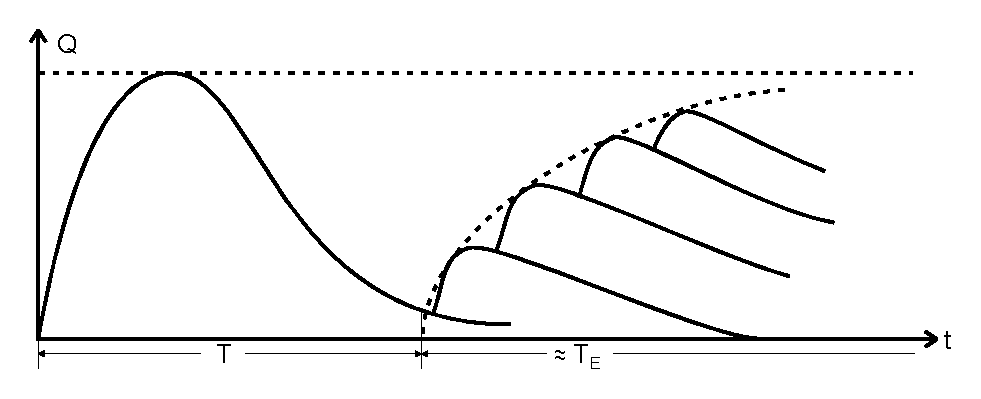
\includegraphics[width=0.8\linewidth]{pictures/Diagramm2.pdf}
    \caption{Tot- und Erholzeit eines Zählrohrs.}\label{fig:Diagramm2}
\end{figure}
Durch die große Masse der positiven Ionen, halten sie sich viel länger im Innenraum auf.
Dadurch wird vorübergehend eine positive, radialsymmetrische Raumladung aufgebaut.
Dieses wird als \textit{Ionenschlauch} bezeichnet.
In dieser Zeit $T$ ist ein eintreffendes Teilchen nicht messbar.
Deshalb wird diese Zeit $T = T_\text{Tot}$ auch \textit{Totzeit} genannt.
Werden die Ionen neutralisiert, folgt eine Erholungszeit $T_\text{Erh}$.
Schematisch ist dies in \hyperref[fig:Diagramm2]{Abbildung \ref{fig:Diagramm2}} dargestellt.
Die Totzeit lässt sich durch die Zwei-Quellen-Methode mit der Gleichung
\begin{equation} \label{eq:T_Tot}
    T_\text{Tot} \approx \frac{\text{N}_1 + \text{N}_2 - \text{N}_{1+2}}{2\text{N}_1 \text{N}_2}
\end{equation}
annähern.
Dabei sind $\text{N}_i$ die Zählraten der Impulse.
Um die Nachentladungen zu reduzieren, wird ein Alkoholzusatz in das Gasgemisch beigefügt.
Dieser neutralisiert die Ionen und reduziert die Elektronenlawinen der positiven Ionen.

\subsection{Charakteristik des Zählrohres}
Werden die gemessene Teilchenzahl N bei konstanter Strahlungsintensität gegen die angelegte Spannung in einem
Diagramm aufgetragen, ergibt sich ein Diagramm wie in \hyperref[fig:Diagramm3]{Abbildung \ref{fig:Diagramm3}}.
Dieses Diagramm wird auch \textit{Charakteristik des Zählrohres} genannt.
Das Plateau beginnt mit der Spannung $U_\text{E}$.
Das Plateau sollte idealerweise die Steigung null haben, jedoch entsteht durch die Nachentladungen (siehe \hyperref[sec:Nachentladungen]{Kapitel \ref{sec:Nachentladungen}})
eine leichte Steigung. Nach dem Plateau entsteht die Dauerentladung der Ionen.
Über den gemessenen Strom an der Anode lässt sich mit der Gleichung
\begin{equation} \label{eq:ladungen}
Z = \frac{I}{e N}
\end{equation}
die freigesetzten Ladungen berechnen. Dabei ist $Z$ die gemessene Teilchenzahl, $e$ die Elementarladung und $N$ die Impulsrate.
\begin{figure}
    \center
    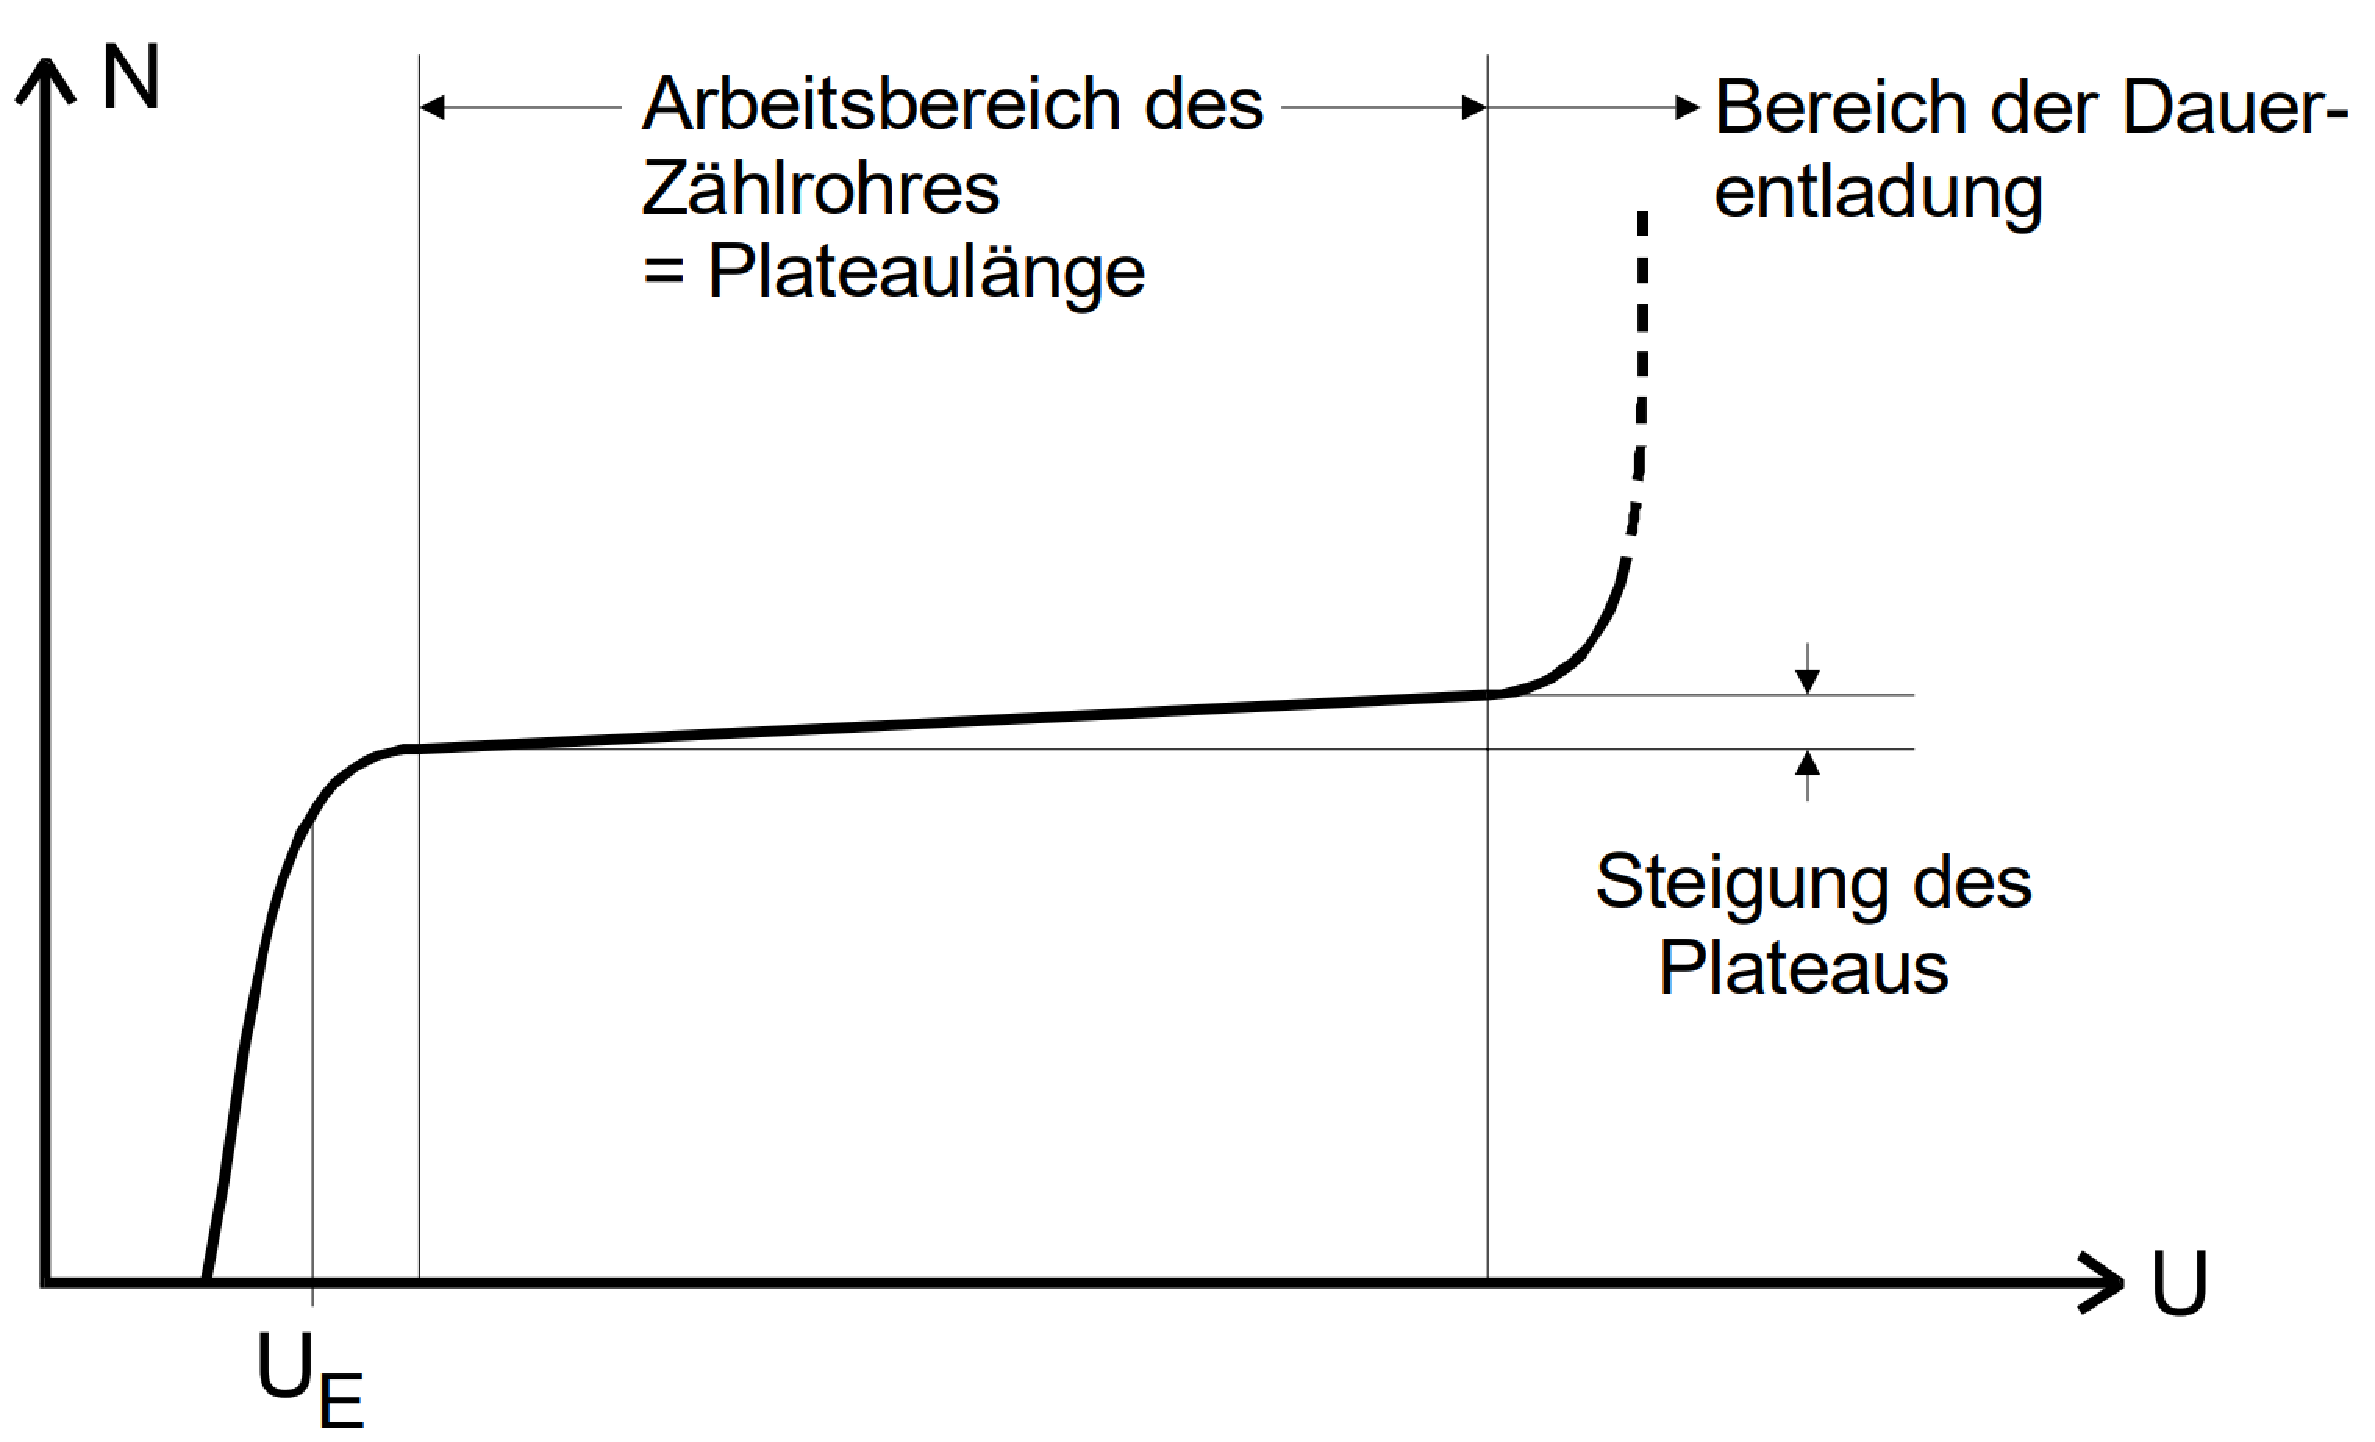
\includegraphics[width=0.7\linewidth]{pictures/Diagramm3.pdf}
    \caption{Charakteristik eines Zählrohres.}\label{fig:Diagramm3}
\end{figure}